\documentclass[journal]{IEEEtran}

\usepackage[T1]{fontenc}
\usepackage[utf8]{inputenc}
\usepackage{amsmath,amssymb,amsfonts}
\usepackage{graphicx}
\usepackage{booktabs}
\usepackage{array}
\usepackage{url}
\usepackage{xcolor}
\usepackage[hidelinks]{hyperref}
\usepackage{orcidlink}
\usepackage{balance}

\graphicspath{{../figures/}}

\renewcommand{\topfraction}{0.92}
\renewcommand{\bottomfraction}{0.75}
\renewcommand{\textfraction}{0.08}
\renewcommand{\floatpagefraction}{0.80}

% IEEEtran hard-codes an em-dash after the abstract and index-terms names; the CAOS
% content standard (ADR-0067) excludes em-dashes, so the separator is a full stop.
\makeatletter
\def\abstract{\normalfont
    \if@twocolumn
      \@IEEEabskeysecsize\bfseries\textit{\abstractname}.\ \relax
    \else
      \bgroup\par\addvspace{0.5\baselineskip}\centering\vspace{-1.78ex}\@IEEEabskeysecsize\textbf{\abstractname}\par\addvspace{0.5\baselineskip}\egroup\quotation\@IEEEabskeysecsize
    \fi\@IEEEgobbleleadPARNLSP}
\def\IEEEkeywords{\normalfont
    \if@twocolumn
      \@IEEEabskeysecsize\bfseries\textit{\IEEEkeywordsname}.\ \relax
    \else
      \bgroup\par\addvspace{0.5\baselineskip}\centering\@IEEEabskeysecsize\textbf{\IEEEkeywordsname}\par\addvspace{0.5\baselineskip}\egroup\quotation\@IEEEabskeysecsize
    \fi\@IEEEgobbleleadPARNLSP}
\makeatother

% Page-1 header block (conventions/manuscript-header-standard.md). The four document
% macros are set by the publishing tool when the version DOI is reserved.
\newcommand{\doctype}{Technical report}
\newcommand{\docversion}{v1.1}
\newcommand{\docdate}{18 September 2026}
\newcommand{\versiondoi}{10.5281/zenodo.22823058}
\newcommand{\conceptdoi}{10.5281/zenodo.21518356}
\newcommand{\docrepo}{github.com/fsantibanezleal/CAOS\_ChancaDEM}
\newcommand{\headerblock}{%
\begin{center}
\fbox{\parbox{0.94\textwidth}{\small\raggedright
\textbf{\doctype} \quad$\cdot$\quad \docversion, \docdate \quad$\cdot$\quad Licence CC BY 4.0\\[2pt]
CAOS open-research programme \quad$\cdot$\quad CAOS\_ChancaDEM, crusher comminution studio\\[2pt]
Version DOI \href{https://doi.org/\versiondoi}{\texttt{\versiondoi}} \quad$\cdot$\quad
concept DOI (always latest) \href{https://doi.org/\conceptdoi}{\texttt{\conceptdoi}}\\[2pt]
Not peer reviewed. Source code, data and computational records: \href{https://\docrepo}{\texttt{\docrepo}}
}}
\end{center}}

\begin{document}

\title{ChancaDEM: A Crusher-Comminution Studio\\ Coupling Whiten, Evertsson and Bond,\\ with a Physics-Faithful Learned Surrogate}

\author{Felipe~Santiba\~nez-Leal~\orcidlink{0000-0002-0150-3246}%
\thanks{F. Santiba\~nez-Leal is with the CAOS open-research programme, Santiago, Chile
(e-mail: fsantibanez@gmail.com; ORCID 0000-0002-0150-3246).}%
\thanks{Interactive studio and reproducible pipeline (MIT) at
\url{https://github.com/fsantibanezleal/CAOS_ChancaDEM}; the studio is available at
\url{https://chancadem.fasl-work.com}.}}

% The leading {} lets IEEEtran's \MakeUppercase reach \doctype, so the whole head is set in capitals.
\markboth{{}\doctype\ \docversion, 2026}%
{Santiba\~nez-Leal: A crusher-comminution studio with a physics-faithful learned surrogate}

\IEEEaftertitletext{\vspace{-0.6\baselineskip}\headerblock\vspace{0.2\baselineskip}}

\maketitle

\begin{abstract}
A rock crusher's product size distribution, throughput and power are governed by well-established comminution
models, but those models are scattered across the literature and rarely coupled in one runnable tool.
ChancaDEM is an interactive studio that couples three cited models, a Whiten classification-breakage population
balance for the product gradation, an Evertsson flow-capacity model for the throughput hump, and Bond's law for
the power, and lets a user set the machine (cone, jaw or gyratory), eccentric speed, throw, closed-side setting
and feed, and see the product form and understand why. On top of the physics engine, a learned surrogate
accelerates it: a multilayer-perceptron trained on the population-balance engine reproduces every output, the
size percentiles, the passing fractions, the throughput and the power, at a coefficient of determination between
$0.980$ and $0.998$ and a mean absolute percentage error of $2.7\%$ to $10.3\%$, on a leakage-safe independent
Latin-hypercube test draw, and, importantly, it preserves the physical monotonicity of product size against
closed-side setting rather than merely fitting the numbers. Over seventeen cases the studio reproduces the
textbook comminution behaviour, coarse high-throughput gyratory products through to fine cone products, and the
classical Bond trade that a finer product costs more specific energy. The studio couples \emph{calibrated models},
not a plant; the surrogate emulates the \emph{engine} and not a real operation; and the three-dimensional chamber
view is a kinematic animation, \emph{not} a discrete-element solve (industrial DEM is infeasible in a browser, and
replaying precomputed DEM traces is left to future work). Every number and figure can be regenerated from the
released artifacts.
\end{abstract}

\begin{IEEEkeywords}
Comminution, crushing, population balance, Whiten model, Bond's law, cone crusher, surrogate model, machine
learning, mineral processing, reproducibility.
\end{IEEEkeywords}

\section{Introduction}

\IEEEPARstart{C}{omminution}, crushing and grinding ore to liberate its minerals, is the largest energy consumer
in a mine, and predicting how a crusher turns a feed into a product is a mature modelling problem~\cite{king}. The
product size distribution follows from a classification-breakage population balance in the tradition of
Whiten~\cite{whiten}, with the breakage described by the JKMRC energy-fineness ($t_{10}$) relation and an
appearance function~\cite{napier}; the throughput follows from the machine's flow capacity, modelled for cone
crushers by Evertsson~\cite{evertsson,quist}; and the power follows from Bond's third theory~\cite{bond}. Each of
these is standard, but a student or an engineer wanting to see how they interact, how eccentric speed, throw and
closed-side setting jointly shape the product, gradation, throughput and power, has to assemble them from
scattered sources. ChancaDEM assembles them into one runnable studio and adds a learned surrogate that makes the
coupled engine instant.

The report describes that studio and, in particular, measures how faithfully the learned surrogate reproduces the
physics engine. Faithfulness is not just goodness-of-fit: a surrogate that fits the training numbers but violates
the monotonic dependence of product size on closed-side setting would be worse than useless in a teaching or
what-if tool, because it would teach the wrong physics. So the surrogate is checked both on accuracy, against a
leakage-safe held-out design, and on physical consistency. The contribution is a coupled,
surrogate-accelerated comminution studio, with the accuracy and the consistency of each part reported, and with
an explicit statement of what the tool is (a coupling of calibrated models) and is not (a plant, or a
discrete-element solve, despite the name).

\section{The Coupled Comminution Engine}\label{sec:physics}

% Defined here so that the full-width float lands at the top of the page where Section III begins.
\begin{figure*}[!t]
\centering
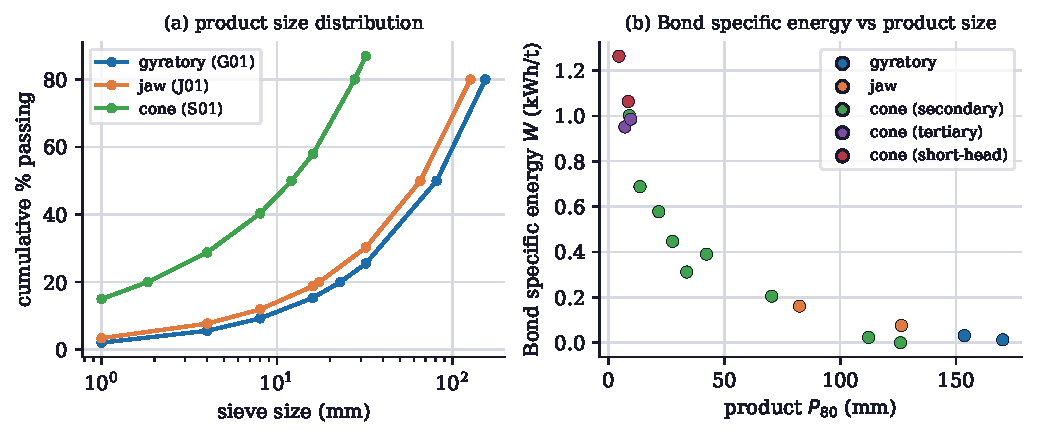
\includegraphics[width=0.84\textwidth]{fig-physics.pdf}
\caption{The coupled engine's response over seventeen cases. \textbf{(a)} Product size distributions (cumulative
percent passing against sieve size) for a gyratory, a jaw and a cone case: the gyratory delivers a coarse
high-tonnage product, the jaw an intermediate one, and the cone a fine product, the size-reduction ladder of a
crushing circuit. \textbf{(b)} Bond specific energy $W$, from which the engine computes the power draw
($P = W\,Q$), against product $P_{80}$ for all seventeen cases, coloured by machine: the finer the product, the
more energy per tonne, the classical Bond trade, from about $0.01$--$0.03$~kWh/t for the coarse gyratory products
to about $1.3$~kWh/t for the finest (short-head cone) product. The two secondary-cone points near zero ($P_{80}$
of 112 and 126~mm) are control settings with the closed side wider than the feed $F_{80}$, which pass the rock
almost unbroken.}
\label{fig:physics}
\end{figure*}

The engine couples three models, all evaluated in closed form so the whole thing runs live. The \textbf{product
gradation} comes from the Whiten classification-breakage population balance~\cite{whiten}: for a feed vector
$\mathbf f$ (mass in size classes), a classification (selection) matrix $\mathbf C$ giving the probability a
particle in each class is broken, and a breakage matrix $\mathbf B$ giving the daughter-size distribution, the
product is
\begin{equation}
\mathbf p \;=\; (\mathbf I - \mathbf C)\,(\mathbf I - \mathbf B\,\mathbf C)^{-1}\,\mathbf f .
\end{equation}
The breakage matrix $\mathbf B$ is built from the JKMRC $t_{10}$ energy-fineness curve (how much fine material a
given breakage energy produces) and an appearance function~\cite{napier}, so the gradation responds physically to
the machine setting. The \textbf{throughput} follows the Evertsson flow-capacity model~\cite{evertsson,quist},
which produces the characteristic unimodal capacity hump against eccentric speed (too slow starves the chamber,
too fast chokes it). The \textbf{power} follows Bond's third theory of comminution~\cite{bond}, the specific
energy scaling with the difference of the inverse square roots of product and feed sizes. The three are coupled:
the same setting that shifts the gradation shifts the capacity and the power, so the studio shows the real
trade-offs a crusher operator faces, not three independent dials.

\section{The Crusher Response}\label{sec:response}

Figure~\ref{fig:physics} shows that the coupled engine reproduces textbook comminution behaviour across
seventeen cases spanning the three machine types. The product size distributions (Fig.~\ref{fig:physics}a) form
the size-reduction ladder of a real circuit: the gyratory crusher produces a coarse product ($P_{80}$ around
$150$~mm) at high throughput (thousands of tonnes per hour), the jaw an intermediate product, and the cone a fine
product ($P_{80}$ under $30$~mm) at lower throughput. The Bond specific energy (Fig.~\ref{fig:physics}b), which
the engine computes from the ore work index and the feed and product sizes and multiplies by the throughput to
obtain the power draw, makes the classical Bond trade visible: across the cases, finer products cost more energy
per tonne, from about $0.01$--$0.03$~kWh/t for the coarse gyratory products to about $1.3$~kWh/t for the finest
short-head cone product, with the primary crushers at the low end (at most $0.16$~kWh/t) and the two short-head
cones at the high end ($1.06$ and $1.26$~kWh/t). None of this is surprising: a studio that couples the cited models should reproduce the
behaviour the models are known to produce, and it does, which is what licenses using it to teach and to explore.

\section{The Learned Surrogate}\label{sec:surrogate}

\begin{figure*}[!t]
\centering
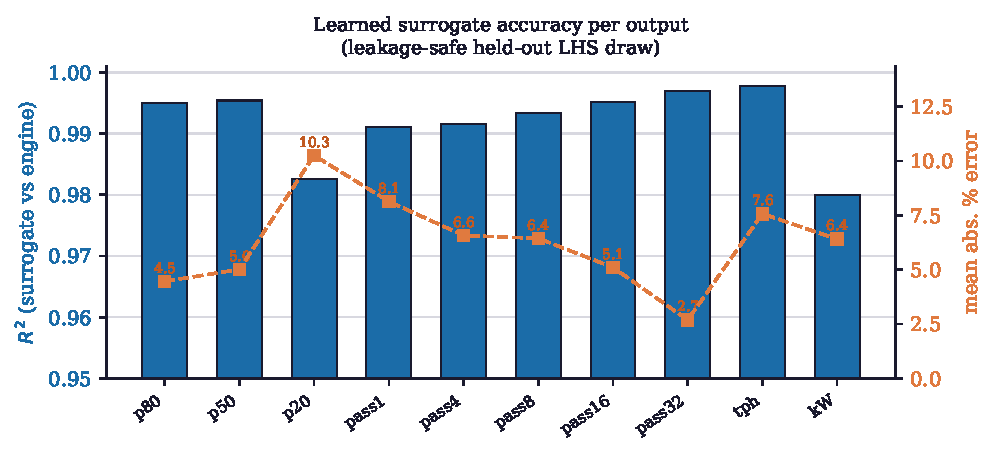
\includegraphics[width=0.80\textwidth]{fig-surrogate.pdf}
\caption{The learned surrogate against the population-balance engine, per output, on a leakage-safe held-out
Latin-hypercube draw (an independent second sampling, not a row split of the training set). The coefficient of
determination (bars) is between $0.980$ and $0.998$ for every output, the product size percentiles, the passing
fractions, the throughput and the power; the mean absolute percentage error (line) is $2.7\%$ to $10.3\%$, worst
on the fine $P_{20}$ tail, as expected. The surrogate also preserves the monotone dependence of $P_{80}$ on
closed-side setting, so it is physically faithful, not just numerically close.}
\label{fig:surrogate}
\end{figure*}

The physics engine is cheap but not instant, and for live what-if exploration the studio runs a learned
surrogate, a multilayer perceptron trained on the population-balance engine to map machine settings and feed to
all ten outputs. Figure~\ref{fig:surrogate} and Table~\ref{tab:surrogate} report its accuracy on a leakage-safe
test set: the held-out data are an independent second Latin-hypercube draw (a different seed), not a random split
of the training rows, so there is no near-duplicate leakage between train and test. On that test the surrogate
reproduces every output at a coefficient of determination between $0.980$ (the power) and $0.998$ (the
throughput), with $0.997$ and $0.995$ for the coarse passing fractions (32 and 16~mm), and a mean absolute
percentage error from $2.7\%$ to $10.3\%$; the
error is largest on $P_{20}$, the fine tail of the product, which is intrinsically the hardest quantity to
predict. Crucially, the surrogate is checked for \emph{physical consistency}, not just fit: it preserves the
monotone increase of product $P_{80}$ with closed-side setting, so it will not teach a user the wrong direction
of a control. A surrogate that is both accurate to a few percent and monotone in the right variables is a faithful
accelerator of the engine; the consistency check is therefore reported alongside the error.

\begin{table}[!t]
\centering
\caption{Surrogate accuracy per output against the population-balance engine (leakage-safe held-out draw,
$n_{\text{test}}=2196$). All outputs $R^2\ge0.980$; the fine $P_{20}$ tail has the largest percentage error.}
\label{tab:surrogate}
\footnotesize
\begin{tabular}{@{}l r r@{}}
\toprule
Output & $R^2$ & MAPE (\%) \\
\midrule
$P_{80}$ (product 80\% size) & $0.995$ & $4.5$ \\
$P_{50}$                     & $0.995$ & $5.0$ \\
$P_{20}$                     & $0.983$ & $10.3$ \\
\% passing 32 mm             & $0.997$ & $2.7$ \\
\% passing 16 mm             & $0.995$ & $5.1$ \\
\% passing 4 mm              & $0.992$ & $6.6$ \\
throughput (tph)             & $0.998$ & $7.6$ \\
power (kW)                   & $0.980$ & $6.4$ \\
\bottomrule
\end{tabular}
\end{table}

\section{Discussion and Scope}\label{sec:discuss}

ChancaDEM is a coupling of established comminution models made interactive, and a demonstration that a learned
surrogate can accelerate such a coupling faithfully, to a few percent and with the physics monotonicity intact.
The value for a learner or an engineer is seeing the three models interact, that the setting which makes the
product finer also moves the capacity hump and raises the power, in one place and in real time, and the surrogate
makes that exploration instant. The studio couples \emph{calibrated models}, not a real plant; the parameters
are physically reasonable but are not fitted to a specific crusher, so the numbers are the models' behaviour, not a prediction for a given machine. The surrogate
emulates the cheap physics \emph{engine}, not a plant, and its accuracy is against that engine. And, despite the
name, the three-dimensional chamber view is a \emph{kinematic animation}, geometry and motion driving the
engine's gradation, and \emph{not} a discrete-element-method solve; industrial DEM of a crushing chamber is
infeasible in a browser, and replaying offline precomputed DEM traces, rather than solving DEM live, is left to
future work. A companion denoising-autoencoder anomaly score flags when the surrogate is asked to extrapolate
outside its training envelope, so a user is warned rather than silently misled. The studio states the same limits
on its methodology pages.

\section{Conclusion}

ChancaDEM couples the Whiten population balance, the Evertsson capacity model and Bond's power law into one
runnable crusher-comminution studio, reproduces the textbook size-reduction ladder and the Bond energy-size trade
across seventeen cases, and accelerates the coupled engine with a learned surrogate that is faithful, coefficient of
determination $0.980$ to $0.998$, error a few percent, and monotone in the right variables. The scope is
calibrated models rather than a plant, a surrogate of the engine rather than of reality, and a kinematic animation
rather than a discrete-element solve; within it, the reproducible coupling and the consistency-checked surrogate
are the contribution.

\appendices
\section{Reproduction}\label{app:repro}

The repository artifacts under \path{data/derived/} carry the seventeen cases' engine outputs
(\path{case-results.json}: gradation, throughput, power and the per-nip breakage energy per case; each case's
\path{trace.json} also records its operating point, including the machine type and the ore work index), the
surrogate metrics (\path{surrogate_metrics.json}: per-output $R^2$ and MAPE on the held-out Latin-hypercube draw,
and the $P_{80}$-monotonicity flag), and the anomaly-detector scaler and threshold. The figure scripts under
\path{manuscripts/comminution-studio/figures/} read those artifacts; Fig.~\ref{fig:physics}b plots the Bond
specific energy as the power divided by the throughput. The physics engine and the surrogate are
deterministic given their inputs, so re-running reproduces Table~\ref{tab:surrogate} and
Figs.~\ref{fig:physics}--\ref{fig:surrogate}.

\balance

\begin{thebibliography}{00}

\bibitem{whiten} W.~J. Whiten, ``The simulation of crushing plants with models developed using multiple spline
regression,'' \emph{Journal of the South African Institute of Mining and Metallurgy}, vol.~72, pp.~257--264,
1972.

\bibitem{napier} T.~J. Napier-Munn, S.~Morrell, R.~D. Morrison, and T.~Kojovic, \emph{Mineral Comminution
Circuits: Their Operation and Optimisation}. Brisbane: Julius Kruttschnitt Mineral Research Centre, 1996.

\bibitem{bond} F.~C. Bond, ``The third theory of comminution,'' \emph{Transactions of the American Institute of
Mining, Metallurgical and Petroleum Engineers}, vol.~193, pp.~484--494, 1952.

\bibitem{evertsson} C.~M. Evertsson, \emph{Cone Crusher Performance}, Ph.D. dissertation, Chalmers University of
Technology, G\"oteborg, Sweden, 2000.

\bibitem{quist} J.~Quist and C.~M. Evertsson, ``Cone crusher modelling and simulation using DEM,'' \emph{Minerals
Engineering}, vol.~85, pp.~92--105, 2016. doi:10.1016/j.mineng.2015.11.004.

\bibitem{king} R.~P. King, \emph{Modeling and Simulation of Mineral Processing Systems}. Oxford:
Butterworth-Heinemann, 2001. doi:10.1016/C2009-0-26303-3.

\end{thebibliography}

\end{document}
